\chapter{Validation}
\label{chapter-3}

%Validation du simulateur avec exo 4 TP 1, sous forme de tableau comparatif à double entrée.....\\
%Détail calcul à la main...\\
%Tracé des rayons obtenus àpd simulateur...\\




Remarque: lors de la simulation de la situation de l'exercice 1 du TP4, nous ne pouvons pas utiliser la puissance sur une zone locale $<P_{RX}>$ (équation \ref{eq:puissance-locale}), mais bien $P_{RX}$ en un point de l'espace (équation \ref{eq:puissance-un-point}).
\begin{equation}
    \label{eq:puissance-un-point}
    P_{RX}\ = \frac{60 \lambda^2}{8 \pi^2 R_a}P_{TX}G_{TX} \left| \sum_{n=1}^N \Gamma_1 \Gamma_2 \Gamma_3 \dotsc T_1 T_2 T_3 \frac{e^{-j \beta d_n}}{d_n} \right|^2
\end{equation}

Le calcul du champ électrique utilise l'équation (\ref{eq:elec-field}).\\

L'exercice 1 du TP4 utilise un $P_{TX}G_{TX}=1.64$, une fréquence à $868.3 \mathrm{MHz}$, une résistance d'antenne $R_a=73 \Omega$, ainsi que des murs ayant comme permittivité relative $\varepsilon_r=4.8$ et comme conductivité $\sigma=0.018 \mathrm{S/m}$.

\section{Calculs pour rayon à deux réflexions, cas A}
La m{\'e}thode pour obtenir les valeurs du cas {\`a} deux r{\'e}flexions est
celle bri{\`e}vement pr{\'e}sent{\'e}e dans la section correspondante, et le
cas {\`a} d{\'e}terminer est d'ailleurs le m{\^e}me que la figure
correspondante.

\subsection{Positions des r{\'e}flexions}

La position des images antenne s'obtient par symétrie, $I_1 = (- 32, 10)$ et
ensuite $I_2 = (- 32, 150)$.
On commence par d{\'e}terminer le point $P_{r 2}$ qui est l'intersection entre
le mur horizontal le plus élevé sur l'axe $y$ (mur B) et $\overrightarrow{I_2 R
X}$. On commence par {\'e}valuer $\overrightarrow{I_2 R X}$ :
\[ \overrightarrow{I_2 R X} = (79, - 85) \rightarrow \| \overrightarrow{I_2 R
   X} \| = 116.04 \rightarrow \frac{\overrightarrow{I_2 R X}}{\|
   \overrightarrow{I_2 R X} \|} = (0.68, 0.73) \]
Avec cela, on peut d{\'e}terminer $P_{r 2}$, dont on conna{\^i}t la
coordonn{\'e}e $y = 80$ et dont on veut d{\'e}terminer la coordonn{\'e}e $x$.
\[ P_{r 2} = I_2 + \frac{\overrightarrow{I_2 R X}}{\| \overrightarrow{I_2 R X}
   \|} t \rightarrow t = 95.56 \rightarrow x = 33.06 \rightarrow P_{r 2} =
   (33.06, 80) \]
Et on peut d{\'e}terminer de la m{\^e}me mani{\`e}re, la coordonn{\'e}e de
$P_{r 1}$, connaissant celle de $P_{r 2}$, le vecteur est donc
$\overrightarrow{I_1 P_{r 2}}$. Nous obtenons
\[ \overrightarrow{I_1 P_{r 2}} = (65.06, 70) \rightarrow \|
   \overrightarrow{I_1 P_{r 2}} \| = 95.57 \rightarrow
   \frac{\overrightarrow{I_1 P_{r 2}}}{\| \overrightarrow{I_1 P_{r 2}} \|} =
   (0.68, 0.73) \]
On connait cette fois ci la coordonn{\'e}e $x = 0$ du point de r{\'e}flexion,
et on cherche $y$.
\[ P_{r 1} = I_1 + \frac{\overrightarrow{I_1 P_{r 2}}}{\| \overrightarrow{I_1
   P_{r 2}} \|} t \rightarrow t = 47 \rightarrow y = 44.43 \rightarrow P_{r 1}
   = (0, 44.43) \]
Il nous reste finalement {\`a} d{\'e}terminer $P_t$ le point d'intersection
entre $\overrightarrow{P_{r 1} \mathrm{TX}}$ et le mur vertical passant par $A =
(0, 20)$.
\[ \overrightarrow{P_{r 1} \mathrm{TX}} = (- 32, 34.43) \rightarrow \|
   \overrightarrow{P_{r 1} \mathrm{TX}} \| = 47 \rightarrow
   \frac{\overrightarrow{P_{r 1} \mathrm{TX}}}{\| \overrightarrow{P_{r 1}
   \mathrm{TX}} \|} = (- 0.68, 0.73) \]
On conna{\^i}t la coordonn{\'e}e $y = 20$,
\[ P_t = \mathrm{TX} + \frac{\overrightarrow{P_{r 1} \mathrm{TX}}}{\|
   \overrightarrow{P_{r 1} \mathrm{TX}} \|} t \rightarrow t = 13.65 \rightarrow
   x = 22.71 \rightarrow P_{r 1} = (22.71, 20) \]

\subsection{Coefficients}

Nous {\'e}valuerons les coefficients en prenant le m{\^e}me ordre que celui du
calcul des points de r{\'e}flexion et transmission. Nous commençons par d{\'e}terminer
$\Gamma_2$ associ{\'e} {\`a} la r{\'e}flexion en $P_{r 2}$, avec la normale est
$(0, - 1)$ nous avons 
\[ \cos \theta_i = \langle \frac{\overrightarrow{I_2 R X}}{\|
   \overrightarrow{I_2 R X} \|}, (0, - 1) \rangle = 0.73 \rightarrow \sin
   \theta_i = \sqrt{1 - \cos^2 \theta_i} = 0.68 \]
L'obtention des composantes transmises dans le mur se font via la loi de
Snell, avec $\varepsilon_r = 4.8$
\[ \sin \theta_t = \frac{1}{\sqrt{\varepsilon_r}} \sin \theta_i = 0.31
   \rightarrow \cos \theta_t = 0.95 \]
La distance parcourue par le rayon dans le mur $s$, est par cons{\'e}quent
\[ s = \frac{l}{\cos \theta_t} = 0.16 \]
Avec $Z_m = (171.57 + 6.65 j){\Omega}$ et $Z_0 = 377 \Omega$, le coefficient
$\Gamma_{\perp}$ de polarisation perpendiculaire vaut
\[ \Gamma_{\perp} = \frac{Z_m \cos \theta_i - Z_0 \cos \theta_t}{Z_m \cos
   \theta_i + Z_0 \cos \theta_t} = - 0.48 + 0.015 j \]
On peut donc, pour finir, {\'e}valuer $\Gamma_2$
\[ \Gamma_m = \Gamma_{\perp} - \frac{(1 - \Gamma_{\perp}^2) \Gamma_{\perp}
   e^{- 2 \gamma_m s} e^{j \beta 2 s \sin \theta_t \sin \theta_i}}{1 -
   \Gamma_{\perp}^2 e^{- 2 \gamma_m s} e^{j \beta 2 s \sin \theta_t \sin
   \theta_i}} = - 0.42 + 0.25 j \]
Les calculs pour $\Gamma_1$ se font de la m{\^e}me mani{\`e}re que
pr{\'e}c{\'e}demment, il nous suffit alors d'indiquer les r{\'e}sultats
interm{\'e}diaires.
Avec le mur de normale $(1, 0)$, on obtient $\cos \theta_i = 0.68$, $\sin
\theta_i = 0.73$, $\sin \theta_t = 0.33$, $\cos \theta_t = 0.94$ et $s = 0.16$.
Qui donnent $\Gamma_{\perp} = - 0.51 + 0.0144 j$, qui permet d'obtenir
\[ \Gamma_1 = - 0.47 + 0.25 j \]
Il nous reste plus qu'{\`a} {\'e}valuer $T_1$ le coefficient de transmission.
Les valeurs trigonom{\'e}triques des angles incidents et transmis sont
facilement obtenables avec la m{\^e}me m{\'e}thode que pr{\'e}c{\'e}demment
$\cos \theta_i = \langle \frac{\overrightarrow{P_{r 1} \mathrm{TX}}}{\|
\overrightarrow{P_{r 1} \mathrm{TX}} \|}, (0, 1) \rangle = 0.73$, $\sin \theta_i
= 0.68$, $\sin \theta_t = 0.31$, $\cos \theta_t = 0.95$ et $s = 0.16$.
Par cons{\'e}quent, $\Gamma_{\perp} = - 0.51 + 0.014 j$ et pour finir
\[ T_1 = \frac{(1 - \Gamma_{\perp}^2) e^{- \gamma_m s}}{1 - \Gamma_{\perp}^2
   e^{- 2 \gamma_m s} e^{j \beta 2 s \sin \theta_t \sin \theta_i}} = 0.63 +
   0.089 j \]

\subsection{Champ et puissance}

L'amplitude du champ se calcule, pour notre cas, via
\[ \underline{E_n} = \Gamma_1 \Gamma_2 T_1 \sqrt{60 P_{\mathrm{TX}}
   G_{\mathrm{TX}}} \frac{e^{- j \frac{2 \pi f}{c} d_n}}{d_n} = 4.4519 \cdot
   10^{- 4} - 2.1816 \cdot 10^{- 5} j \]
Avec la distance $d_n$ {\'e}tant celle qui s{\'e}pare $\mathrm{RX}$ de
$\mathrm{TX}$, c'est aussi la distance qui s{\'e}pare $\mathrm{RX}$ de $I_2$, et
vaut donc $\| \overrightarrow{I_2 R X} \| = 116.04$.
\\
La puissance vaut donc
\[ P_{RX} = \frac{60 \lambda^2}{8 \pi^2 R_a} P_{TX} G_{TX} \left| \Gamma_1 \Gamma_2 T_1  \frac{e^{- j \beta d_n}}{d_n} \right|^2
   = 4.1145 \cdot 10^{- 12} W \]
Ce qui donne, en $\mathrm{dB}$, $< P_{\mathrm{RX}} > = - 83.85 \mathrm{dBm}$.


\section{Comparaison calculs et simulation}
Nous pouvons comparer les résultats de notre simulateur avec les résultats calculés manuellement afin de valider notre implémentation. Un tableau comparatif [Table \ref{tab:comparaison-calculs-simulation}] présente ces données.

\begin{table}[H]
    \centering
    \begin{tabular}{|l|l|r|r|r|}
         \hline
                                  & Grandeur & Calculs & Simulation & Erreur \\
        \hline
\multirow{2}{*}{Direct}           & $\left|\underline{E}\right|$ [V/m] & $4,031\cdot10^{-3}$ & $4,0124\cdot10^{-3}$ & $0,40\%$ \\
                                  & $P_{RX}$ [W] & $3,33\cdot10^{-10}$  & $3,32965\cdot10^{-10}$ & $0,01\%$     \\
        \hline
\multirow{2}{*}{1 réflexion (A)}  & $\left|\underline{E}\right|$ [V/m] & $7,0819\cdot10^{-4}$ & $7,07611\cdot10^{-4}$ & $0,08\%$ \\
                                  & $P_{RX}$ [W] & $1,04\cdot10^{-11}$ & $1,03557\cdot10^{-11}$ & $0,42\%$ \\
        \hline
\multirow{2}{*}{1 réflexion (B)}  & $\left|\underline{E}\right|$ [V/m] & $6,7821\cdot10^{-4}$ & $6,78351\cdot10^{-4}$ & $0,02\%$ \\
                                  & $P_{RX}$ [W] & $9,53\cdot10^{-12}$ & $9,51694\cdot10^{-12}$ & $0,14\%$ \\
        \hline
\multirow{2}{*}{2 réflexions (A)} & $\left|\underline{E}\right|$ [V/m] & $4,4572\cdot10^{-4}$ & $4,46271\cdot10^{-4}$ & $0,12\%$ \\
                                  & $P_{RX}$ [W] & $4,1145\cdot10^{-12}$ & $4,11896\cdot10^{-12}$ & $0,11\%$ \\
        \hline
%\multirow{2}{*}{2 réflexions (B)} & $\left|\underline{E}\right|$ [V/m] &   N/A   &      & N/A    \\
%                                  & $P_{RX}$ [W] &   N/A   &      & N/A    \\
%         \hline
    \end{tabular}
    \caption{Comparaison valeurs calculs et simulation selon le rayon}
    \label{tab:comparaison-calculs-simulation}
\end{table}

On peut observer que notre simulateur se rapproche beaucoup des valeurs réelles calculées à la main, avec une erreur ne dépassant pas 0,5\%. Ceci permet donc de valider l'implémentation de notre simulateur.

\section{Affichage simulation des rayons}

La Figure [\ref{fig:simu-tp4}] présente le tracé des rayons simulés. Le récepteur est représenté comme un carré bleu, l'émetteur comme un rond blanc, les points de réflexions comme des points magenta, les murs comme des traits gris, et les rayons sont différenciés par leur couleur représentant leur nombre de réflexions:
\begin{itemize}
    \item Vert: rayon direct (0 réflexion)
    \item Rouge: rayon à une réflexion
    \item Jaune: rayon à deux réflexions
\end{itemize}

\begin{figure}[H]
    \centering    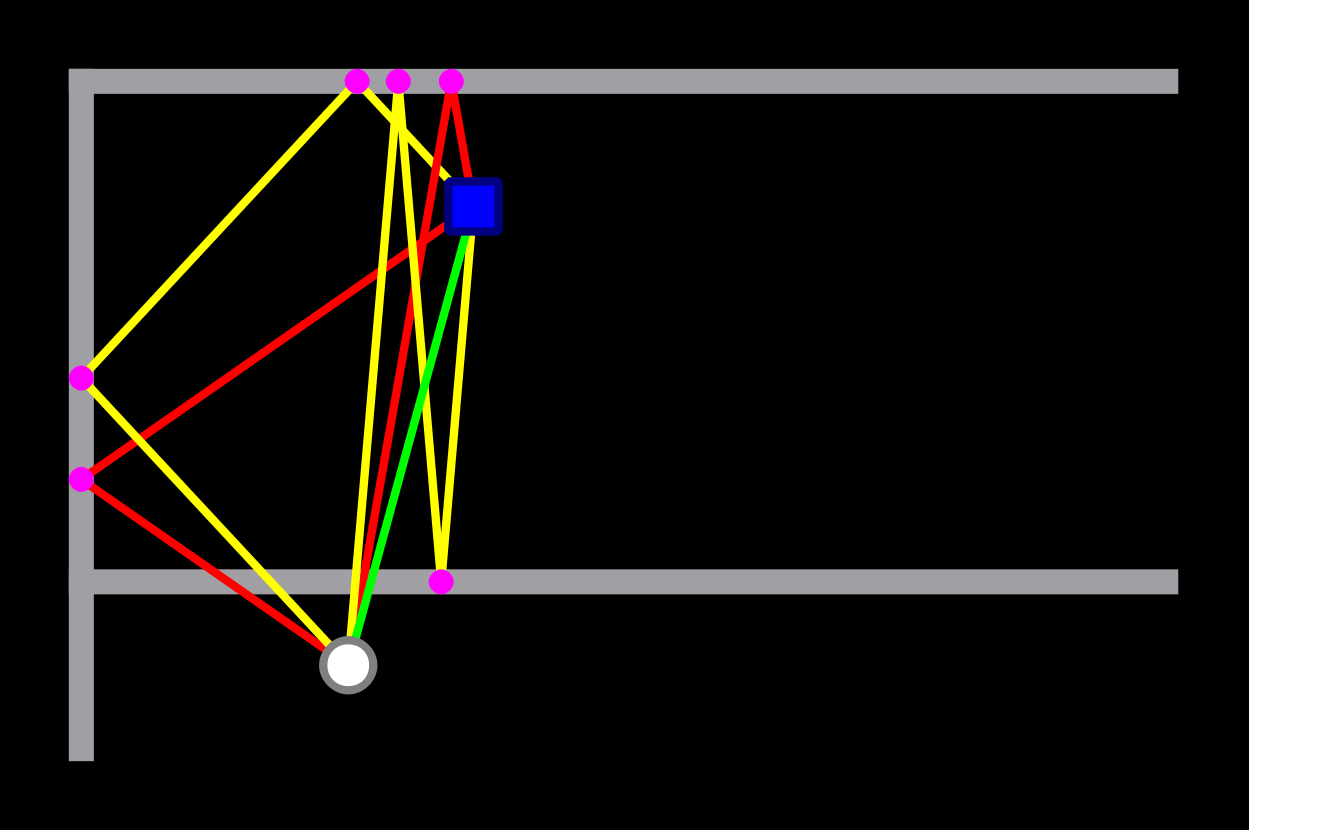
\includegraphics[width=\textwidth]{latex/images/tp4.png}
    \caption{Simulation Ray-Tracing de l'exercice 1, TP4}
    \label{fig:simu-tp4}
\end{figure}

Comme le simulateur complet de l'appartement, il est possible d'afficher plus d'informations du récepteur, tel que ses coordonnées ou encore sa puissance reçue, lors du survol de la souris par-dessus.
